\section{Results Discussion}

\subsection{Training}

% Arguments:

Figure~\ref{fig:q-values} shows the different performances from the 4 configurations. In order to reduce the noise of the Q-value estimates, as the cited papers did, during the training \auth~take the averages of the Q-values from \numepoch~steps, defined as \textit{epoch}. %More epochs computed by a configuration implies more steps per episode and then more reward in general. Hence the \textit{deep} configurations played better than the \textit{shallow}. More details in the evaluation subsection.

An interesting viewpoint is the overestimation issue. If the reward is nonzero and $\gamma < 1$ as in the \textit{CartPole} environment the return $G_t$ is $\frac{1}{1 - \gamma}$ \cite{Sutton:1998:IRL:551283}. Hence in \authpp~case the return with $\gamma = 0.99$ is $100$ then the DQN has to converge to that value.
Figure~\ref{fig:q-values} shows that the \textit{shallow} configurations converge to 100. Instead the \textit{deep} configurations after about 400 epochs started to oscillate and to overestimate the true return. \Auth~think the \textit{deep} configurations failed to generalize and suffers of overfitting.

In spite of the expectation the Double Q-learning did not reduce significantly the overestimation, the differences between the \textit{shallow} configurations are minimal. Both the \textit{deep} configurations suffer of overestimation, in particular in the last epochs.

\begin{figure*}[]
	\centering
	\subfloat{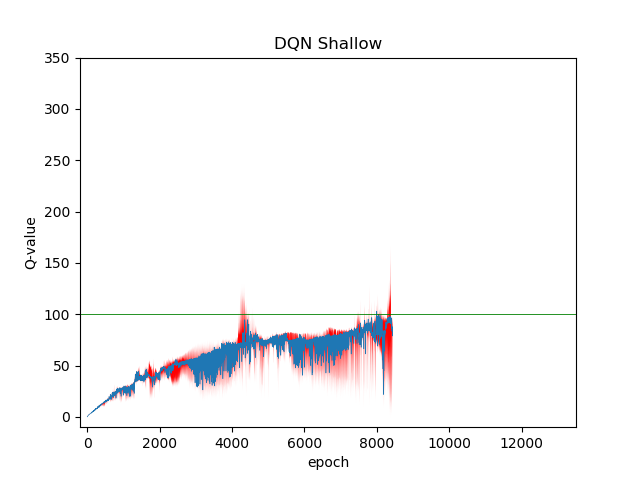
\includegraphics[width=.48\textwidth]{res/DQN_Shallow}} \quad
	\subfloat{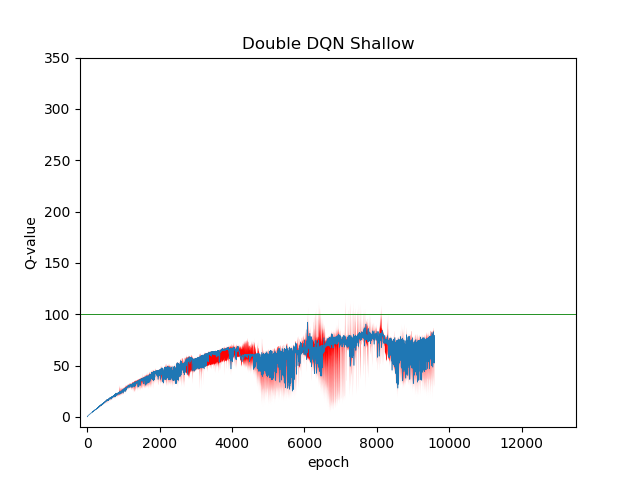
\includegraphics[width=.48\textwidth]{res/DoubleDQN_Shallow}} \\
	\subfloat{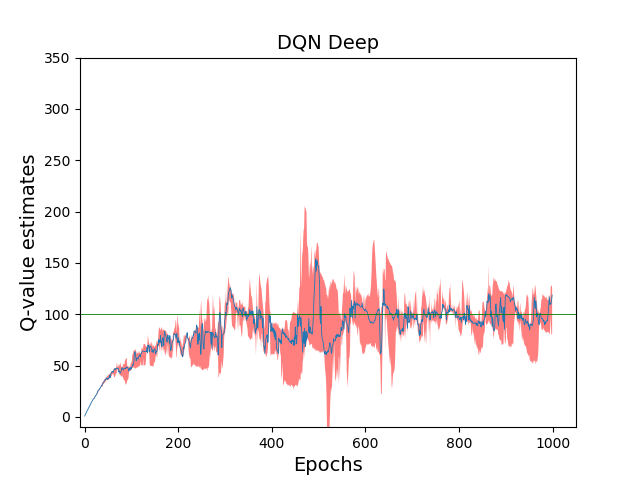
\includegraphics[width=.48\textwidth]{res/DQN_Deep}} \quad
	\subfloat{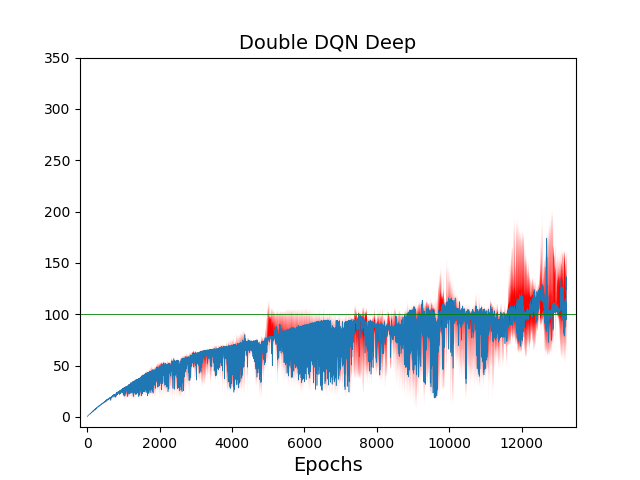
\includegraphics[width=.48\textwidth]{res/DoubleDQN_Deep}} \\
	
	%\subfloat[][\emph{Cascata}.]
	%{\includegraphics[width=.45\textwidth]{Cascata}} \quad
	%\subfloat[][\emph{Salita e discesa}.]
	%{\includegraphics[width=.45\textwidth]{SalitaDiscesa}}
	\caption{The plots shows the Q-value estimates performance for each configuration running for about 1 Million of steps. %Each episode performs every step depending on the good or bad interaction of the agent. This means that some agent finished in less steps.% 
	Each point on the blue lines is the median Q-value per epoch (the average Q-value computed every \numepoch~steps) of 3 executions with different seed. The red area shows the maximum and minimum Q-value per epoch of 3 executions with different seed.}
	\label{fig:q-values}
\end{figure*}


\subsection{Evaluation}

% Theses:
The results of evaluation (Figure~\ref{fig:comparison}) of the model show that the \textit{double} configurations have better results in terms of number of episodes necessary to solve the \textit{CartPole} problem. The DDQN shallow and DDQN deep configurations obtained after 200 and 300 episodes are able to \textit{solve} the \textit{CartPole} problem. It is a good result considering that the algorithm hyperparameters were not tuned. Notice that \auth~consider the best model from 3 run with different seed. 

\begin{figure}[t]
	\centering
	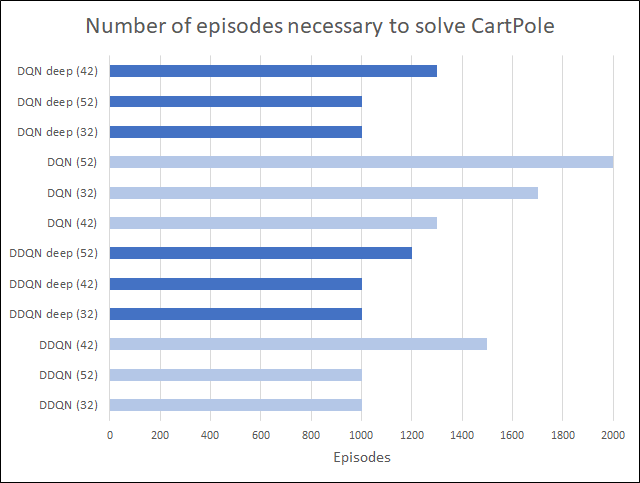
\includegraphics[width=0.46\textwidth]{res/Comparison}
	\caption{Number of episodes necessary to solve the \textit{CartPole} problem for each configuration. The value is selected from the best runs.}
	\label{fig:comparison}
\end{figure}

In fact from the Table~\ref{tab:comparison_table} emerges that a different seed could imply a good or a bad learning process. The \textit{DQN shallow} configuration showed that for the best seed it needs 400 episodes in order to solve the problem while with the seed 52 it needs 1700 episodes. Probably this is caused by a great component of randomness in the DQN algorithm: the probability involves in \textit{$\epsilon$-greedy}, the random selection of mini-batches from the \textit{experience replay} dataset, the random initialization of the parameter of the Q-network and the randomness in the environment.

Another interesting result is that the agent when learn to solve the problem, get 200 as reward, after some good episodes it returns to perform poorly. The Table~\ref{tab:comparison_table} shows that only about 1/4 of the 83 models solved the problem, this means that more episodes of training does not mean better agent performance.

\begin{table}
	\centering
	\begin{tabular}{|c|c|c|c|}
		\hline
		\textbf{Configuration} & \textbf{Seed} & \textbf{Good models} & \textbf{Solved (Ep.)} \\
		\hline
			 & 32 & 13 / 83 & 300 \\
		DDQN shallow & 42 & 16 / 83 & 600 \\
			 & 52 & 16 / 83 & 300 \\
		\hline
		 		& 32 & 21 / 83 & 400 \\
		DDQN deep  & 42 & 20 / 83 & 200 \\
				  & 52 & 17 / 83 & 200 \\
		\hline
					& 32 & 26 / 83 & 400 \\
		DQN	shallow & 42 & 18 / 83 & 1000 \\
					& 52 & 16 / 83 & 1700 \\
		\hline
				 & 32 & 20 / 83 & 500 \\
		DQN deep & 42 & 21 / 83 & 1000 \\
				 & 52 & 25 / 83 & 400 \\
		\hline
	\end{tabular}
	\caption{Results from evaluation. For each configuration with a seed, a model every 100 episode was evaluated. Good models represent the number of models that solved the \textit{CartPole} problem. Solved column shows the number of episodes necessary for obtaining the first good model.}
	\label{tab:comparison_table}
\end{table}
